\chapter{Probabilidad y Estadística}

\section{Probabilidad}
% Página 67 del cuaderno en papel

Los sucesos en probabilidad se escriben entre comillas y se representan con una letra mayúscula.

\begin{itemize}
    \item[m] $I =$ impar
    \item[m] $I =$ probabilidad de sacar un número impar
    \item[m] $I =$ "Probabilidad de sacar un número impar"
    \item[b] $I =$ "Sacar un número impar"
\end{itemize}

\textbf{Operaciones con conjuntos (o sucesos)}

$A\cup B = \{x\in A \vee x \in B\}$ (Unión)

$A\cap B = \{x\in A \wedge x \in B\}$ (Intersección - Probabilidad compuesta)

$A^c = \overline{A} = \{x\not\in A$ (Complementario) \textit{No se llama contrario}.

$A - B = \{x\in A \wedge x \not\in B\}$ (Diferencia)

\obs $A - B = A \cap \overline{B}$

\begin{defn}[Leyes\IS de de Morgan]
\[\overline{A\cap B} = \overline{A}\cup \overline{B}\]
\[\overline{A\cup B} = \overline{A}\cap \overline{B}\]
\end{defn}



\begin{defn}[Compatibilidad]
Sean $A,B$ dos sucesos.

Son compatibles si $A\cap B \not= \emptyset$. 
Son incompatibles si $A\cap B =\emptyset$
\end{defn}

\begin{defn}[Sistema completo de sucesos]
Sean $A_1,...,A_n$ sucesos de un cierto experimento aleatorio.
%
Se dice que forman un sistema completo de sucesos del espacio muestral $E$ cuando:

\begin{itemize}
    \item $\displaystyle\bigcup_{i=1}^n A_i = A_1\cup A_2 \cup ... \cup A_n =  E$
    \item $A_i\cap A_j = \emptyset\;\;\; \forall i,j=1...n$
\end{itemize}
\end{defn}

\begin{example}
Sea $E = \{1,2,3,4,5,6\}$. ¿Son sistemas completos de sucesos las siguientes agrupaciones?

\begin{itemize}
    \item $A_1 = \{1,2,3\}; A_2 = \{4,5\} ; A_3 = \{6\}$
    \item $A_1 = \{\text{múltiplos de 3}\} ; A_2 = \{\text{números pares}\} ; A_3 = \{1,5\}$
\end{itemize}
\end{example}


\begin{prop}Sea $A_1,...,A_n$ un sistema completo de sucesos. Entonces \[\displaystyle\sum_{i=1}^n P(A_i) = 1\]
\end{prop}


\begin{defn}[Regla de Laplace]
Si los socesos elementales de un experimento aleatorio son equiprobables, entonces, $P(A) = \frac{\text{casos favorables}}{\text{casos posibles}}$
\end{defn}
\obs ¿Y si no son equiprobables? 

\begin{defn}[Probabilidad\IS Ley de los grandes números]
Sea $A$ un suceso y $h(A)$ su frecuencia de ocurrencia relativa\footnote{El porcentaje de veces que ese suceso ocurre.} en $n$ repeticiones del experimento. Entonces \[P(A) = \lim_{n\leftrightarrow \infty}h(A)\]
\end{defn}


\begin{defn}[Probabilidad\IS Axiomática de Kolmogorov]
    Sea $p$ una función que asocia a cada suceso $A$ del espacio de sucesos $S$ un número real designado por $p(A)$.
    
    Decimos que $p$ es una probabilidad si cumple las siguientes propiedades:
    \begin{itemize}
        \item $0\leq p(A) \leq 1 \;\;\;\forall A\in S$
        \item $p(E) = 1$
        \item $A\cap B = \emptyset \implies p(A\cup B) = p(A) + p(B)$
    \end{itemize}
\end{defn}

\paragraph{Propiedades de la probabilidad:} Sea $A$ un suceso cualquiera:
\begin{itemize}
    \item $P(\overline{A}) = 1 - P(A)$
    \item $A\subset B \implies P(A) \leq P(B)$
    \item $0\leq P(A) \leq 1$
    \item $P(A\cup B) = P(A) + P(B) - P(A\cap B)$
\end{itemize}

\begin{center}
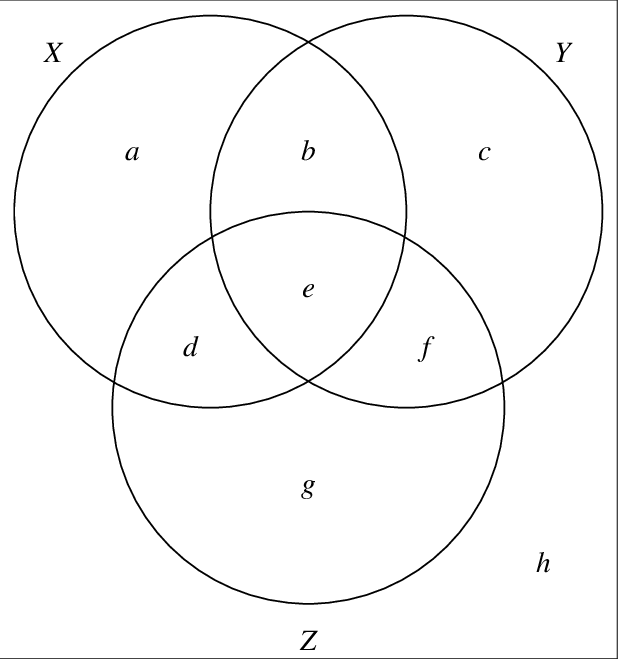
\includegraphics[scale=0.3]{img/Venn-diagram-visualization-of-a-3-event-probability-space-O.png}
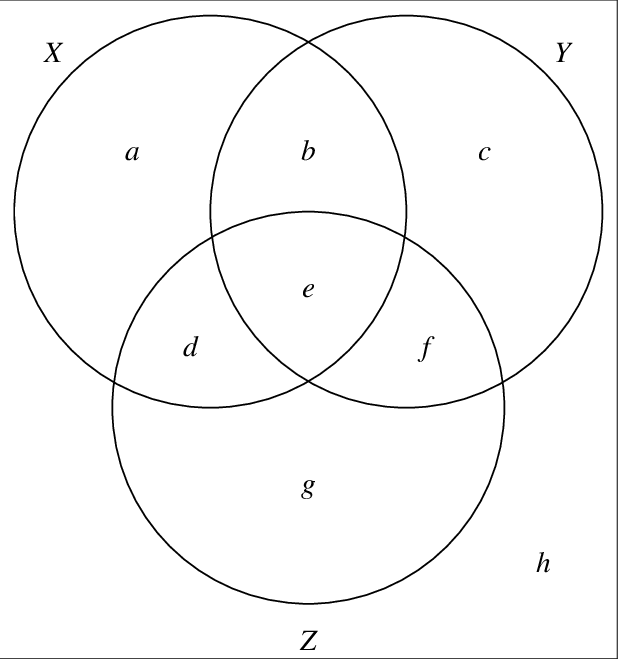
\includegraphics[scale=0.3]{img/Venn-diagram-visualization-of-a-3-event-probability-space-O.png}
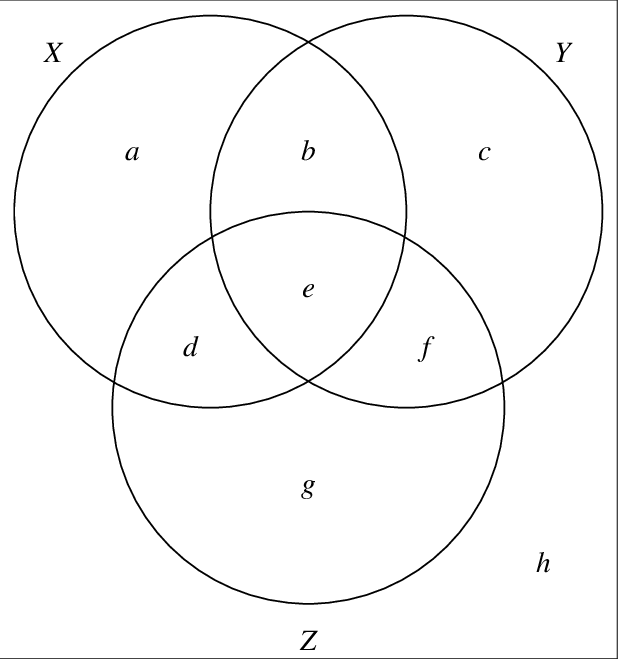
\includegraphics[scale=0.3]{img/Venn-diagram-visualization-of-a-3-event-probability-space-O.png}
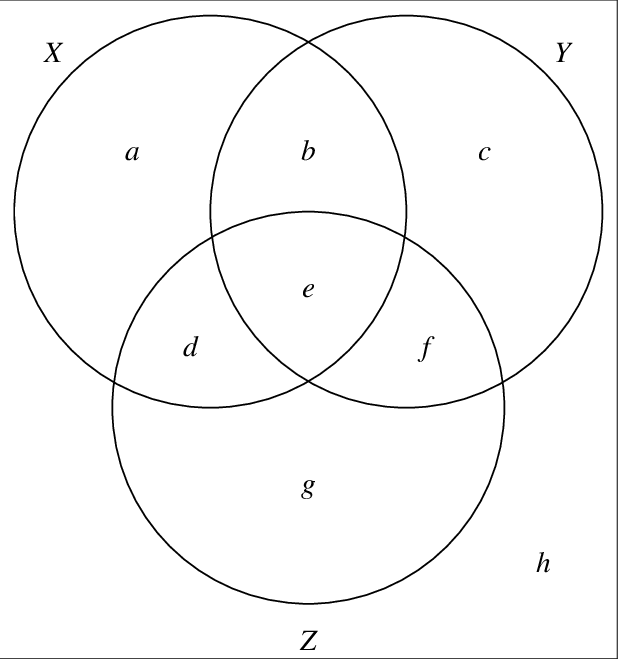
\includegraphics[scale=0.3]{img/Venn-diagram-visualization-of-a-3-event-probability-space-O.png}
\end{center}

\begin{defn}[Probabilidad\IS condicionada]
Sean $A,B$ sucesos de un suceso aleatorio. 

Se define la probabilidad condicionada $p(A/B)$ como la probablidad de que se produzca $A$ si sabemos que se ha producido $B$.

\[P(A/B) = \frac{P(A\cap B)}{P(B)}\]
\end{defn}

\textit{Este es un buen momento para hacer algún ejercicio. Página 349, ejer 36 por ejemplo. Recordamos que $P(A\cup B) = P(A) + P(B) - P(A\cap B)$}

\begin{defn}[Independencia de sucesos]
$A,B$ son sucesos independientes si y sólo si \[P(A/B) = P(A/\overline{B}) = P(A)\]
\end{defn}

\begin{theorem}
\[A,B \text{ independientes } \dimplies P(A\cap B) = P(A)·P(B)\]
\end{theorem}
\begin{proof}
\[\left.\begin{array}{c}
P(A/B) = \frac{P(A\cap B)}{P(B)} \dimplies P(A\cap B) = P(B)·P(A/B)\\A,B \text{ independientes } \dimplies P(A/B) = P(A)\end{array}\right\}*\]
\[(*) \implies P(A\cap B) = P(B)·\underset{P(A/B)}{P(A)} = P(B)·P(A)\]
\end{proof}

\begin{theorem}[Teorema\IS Probabilidad Total]
Sea $A_1,A_2,...,A_n$ un sistema completo de sucesos y sea $B$ otro suceso.
\[  
    P(B) = P(A_1\cap B) + P(A_2\cap B) + ... + P(A_n\cap B) = 
\]
\[
    P(B/A_1)·P(A_1) + P(B/A_2) · P(A_2) + ... + P(B/A_n)·P(A_n)
\]
\end{theorem}
\begin{theorem}[Teorema\IS de Bayes]
\[P(B/A) = \frac{P(A/B)·P(B)}{P(A)}\]
\end{theorem}
\begin{proof}
\[
\left.
\begin{array}{c}
    P(A\cap B) = P(A)·P(B/A)\\
    P(A\cap B) = P(B)·P(A/B)
\end{array}\right\} \implies P(A)·P(B/A) =  P(B)·P(A/B) \dimplies \]\[\dimplies P(B/A) = \frac{P(A/B)·P(B)}{P(A)} 
\]
\end{proof}


\paragraph{Bayesian trap (obtenido de youtube.com/Veritasium)}

\begin{example}
Se sabe que una enfermedad rara sólo afecta al 1\% de la población. 
%
El porcentaje de falsos positivos de las pruebas médicas es del 10\%, y el porcentaje de falsos negativos es del 1\%.

Intuitivamente, ¿cuál dirías que es la probabilida de tener la enfermedad sabiendo que has dado positivo en el test? ¿Podrías calcularlo numéricamente?

Los datos son: $P(E) = 0.01$, $P(-|E) = 0.01$ y $P(+|\overline{E})=0.1$

Aplicando el teorema de Bayes:

\[P(E|+) = \frac{P(+|E)·P(E)}{P(+)} = \frac{P(+|E)·P(E)}{P(+|E)·P(E) + P(+|\overline{E})·P(\overline{E})}= 0.01 \]
\end{example}


\section{Estadística}

A la hora de hacer un estudio estadístico buscamos obtener información sobre toda la población. A veces, esa cantidad de información es inmanejable e inconseguible. 
%
Por ejemplo, test de COVID a toda la población para ver cuántos lo han pasado, no es viable. 
%
Por ello, se selecciona una parte de la población y se le hacen los test a una parte para después extrapolar esos resultados.

Así, definimos:

\begin{defn}[Población]
\end{defn}

\begin{defn}[Muestra]
\end{defn}

\begin{defn}[Individuo]
\end{defn}

\textit{Nota: estos términos también se utilizan al tratar de tornillos en una fábrica.}

Este año vamos a trabajar y a distinguir los \concept[Parámetros\IS poblacionales]{parámetros poblacionales} de los \concept[Parámetros\IS muestrales]{muestrales}.
%
Llamaremos $\mu$ y $\sigma·$ a la media y desviación típica \emph{poblacionales} y $\bar{x}$ y $S$ a la media y desviación típica \emph{muestral}.

El \textbf{objetivo} de este tema es conseguir información sobre los parámetros poblacionales a partir de los parámetros muestrales. 

Para ello, antes de empezar es necesario que intentemos contestar la pregunta: ¿Cómo se asegura uno de que su muestra es buena? Porque si queremos saber lo que opinan los alumnos del colegio sobre la semipresencialidad y tomamos de muestra a los alumnos de 2º de Bachillerato, la información que saquemos no será fiable.

Necesitaremos que las muestras sean \concept[Representatividad de una muestra]{representativas} de toda la población, esto es, que refleje fielmente las características de la población.
%
Llamamos \concept{muestreo} al proceso por el que se construye una muestra de una población. 
%
Como seguro que te imaginas, hay distintos tipos de \textit{muestrear} una población. Vamos a verlos:

\subsection{Tipos de muestreo}

Los muestreos pueden ser aleatorios (si todos sus miembros tienen la misma posibilidad de ser elegidos) o no aleatorios (si no es así).
%
Dado que los muestreos aleatorios otorgan una mayor representatividad, nos centraremos en ellos:

Consideremos que eres el encargado de calidad de una fábrica de tornillos, que fabrica tornillos de distintos tipos.

\begin{itemize}
    \item Aleatorio simple.
        \subitem ¿Cuántas muestras se pueden formar?
        \subitem Estimación de los parámetros poblacionales desde los muestrales.
        \subitem Con reposición (días de la semana que se tienen que elegir), sin reposición (personas).
    \item Sistemático.
    \subitem Ordenados, de h en h (\concept{Constante de elevación}).
    \item Estratificado:
    \subitem Agrupación por característica. Estratos diferentes entre ellos. Elementos iguales en cada estrato.
    \subitem Afijación igual o proporcional.
    \subitem Dentro de cada estrato... ¿Aleatorio simple? ¿Sistemático?
    \item Conglomerados:
    \subitem División de cada característica. Conglomerados iguales entre ellos. Elementos diferentes en cada estrato.
    \subitem Dentro de cada estrato... ¿Aleatorio simple? ¿Sistemático?
\end{itemize}


\textbf{Importancia de los grupos control}

\section{Distribuciones de probabilidad}

Repaso de la distribución normal desde el PPT del departamento.
% 
\section{Inferencia estadística}

Inferir significa deducir algo o sacarlo como conclusión de otra cosa. \footnote{\href{https://dle.rae.es/inferir}{https://dle.rae.es/inferir}}

La tarea que nos va a mantener ocupados unas semanas va a ser la siguiente: \textit{Disponemos de una población con un parámetro desconocido. Tomaremos una muestra e inferiremos acerca del valor del parámetro poblacional utilizando información sobre la muestra.}


\subsection{Inferencia sobre la media}

Trabajaremos haciendo inferencia de la media. 
%
Tendremos poblaciones de las que conocemos su desviación típica (irreal en la vida diaria, pero así es el mundo de 2º de Bachillerato). Más adelante, en vuestra historia con las matemáticas, haréis inferencia de una manera más seria.

\begin{example}
Los de casa, rellenad en el enlace que os doy vuestro dato sobre la altura. Nuestra población serán todos los alumnos que están en casa. 

Una vez dispongamos de los datos, vamos a tomar una muestra para estimarla media de la población. ¿De cuánto cogemos la muestra? De cuantas más personas, mejor, ¿no?

 Hay un resultado fundamental en inferencia estadística (Teorema Central del Límite) del que se deduce que la \concept[Distribución de la media muestral]{media muestral se distribuye} $\overline{X} \sim N\left(\mu,\frac{\sigma}{\sqrt{n}}\right)$
\end{example}

\begin{example}
Ejemplo de cálculo, siguiendo el libro.
\end{example}

\subsubsection{Estimación de la media}
Lo que acabamos de hacer no es inferir, sino entender que la media muestral se distribuye según una distribución normal cuando tenemos suficientes datos (>30) o los datos poblacionales siguen una distribución normal. 

¿Qué ocurre si desconocemos la media de la población y queremos inferirla con una muestra?
%
Tenemos \textbf{dos opciones}, estimación puntual y estimación por intervalos.

\subparagraph{Estimación puntual: } Inferimos $\mu$ a partir de $\overline{X}$ y decimos: $\mu \sim \overline{X}$

\subparagraph{Estimación por intervalos de confianza: } Inferimos $\mu$ a partir de $\overline{X}$ y $\sigma$ y decimos: $\overline{X} - E < \mu < \overline{X} + E$, donde $E$ es una amplitud del intervalo que dependerá de varios factores:
\begin{itemize}
    \item \textbf{La confianza:} no hay ninguna duda que $-\infty<x<\infty$. Esta inferencia tiene una confianza del 100\%, pero no da mucha información. 
    \item \textbf{La desviación típica poblacional $\sigma$:} ya que, cuanto más dispersos estén los datos de la población, más variabilidad tendrá $\overline{X}$ y más grande deberá ser el intervalo para la misma confianza.
\end{itemize}

\begin{theorem}[Intervalo de confianza para la media]

Un intervalo de confianza para la media población de una distribución normal con desviación típica conocida, con un nivel de confianza $1-\alpha$ construido a partir de una muestra de tamaño $n$ es:
\[\left(\overline{x} - \mathcal{E} , \overline{x} + \mathcal{E}\right)\]



Donde $\mathcal{E} = z_{\rfrac{\alpha}{2}}·\frac{\sigma}{\sqrt{n}}$ y se denomina \concept{Error máximo admisible} (no es otra cosa que la amplitud del intervalo de confianza).

Y $\zalfamedios$ es el valor que cumple:
\[ P(\left -\zalfamedios < Z < \zalfamedios\right) = 1-\alpha\]

\obs Nivel de confianza $1-\alpha$ $\dimplies$ Nivel de significación $\alpha$
\end{theorem}

\begin{example}
Ejemplo de cálculo sacado del libro.
\end{example}

\paragraph{Ejercicio 11}

\paragraph{Cálculo del tamaño de la muestra: } Dado que $\mathcal{E} = z_{\rfrac{\alpha}{2}}·\frac{\sigma}{\sqrt{n}}$, podríamos buscar qué tamaño de la muestra debo escoger para construir un intervalo de confianza de amplitud dada.

\begin{example}
Ejemplo de cálculo del libro.
\end{example}

\textbf{Ejercicio 16}

\subsection{Inferencia sobre la proporción}

Lo primero que necesitamos tener claro es lo que es una \concept{proporción}:


\newcommand{\matp}{\rho}
Llamaremos $\hat{P}$ a la distribución de la proporción meustral. Será $\matp$ el parámetro a estimar.

\[\hat{P} \sim N\left(\matp,\sqrt{\frac{\matp q}{n}}\right), q=1-\matp\]

\begin{example}
Ejemplo de cálculo del libro
\end{example}

\subsubsection{Estimación sobre la proporción}

Aquí también tenemos la estimación puntual $\left(\hat{P} \approx \matp\right)$ y una estimación por intervalos de confianza.


\begin{prop}[Intervalo de confianza para la proporción]

Un intervalo de confianza para la proporción de individuos que cumplen una característica en una población, con un nivel de confianza $1-\alpha$ construido a partir de una muestra de tamaño $n$ es:
\[\left(\hat{p} - \mathcal{E} , \hat{p} + \mathcal{E}\right)\]



Donde $\mathcal{E} = z_{\rfrac{\alpha}{2}}·\sqrt{\frac{\hat{p}\hat{q}}{n}}$ y se denomina \concept{Error máximo admisible} (no es otra cosa que la amplitud del intervalo de confianza).

Y $\zalfamedios$ es el valor que cumple:
\[ P(\left -\zalfamedios < Z < \zalfamedios\right) = 1-\alpha\]

\obs Nivel de confianza $1-\alpha$ $\dimplies$ Nivel de significación $\alpha$
\end{prop}

\begin{example}
Ejemplo de cálculo del libro
\end{example}

\textbf{Ejercicio 17}

\paragraph{Cálculo del tamaño de la muestra: } Dado que $\mathcal{E} = z_{\rfrac{\alpha}{2}}·\sqrt{\frac{\hat{p}\hat{q}}{n}}$, podríamos buscar qué tamaño de la muestra debo escoger para construir un intervalo de confianza de amplitud dada.

\begin{example}
Ejemplo de cálculo del libro.
\end{example}

\textbf{Ejercicio 19}